\section{Epilogue}
     \begin{frame}[t]{Epilogue}\framesubtitle{Schedule}
        \begin{itemize}
            \item Improvements on Current Work
            \item Conclusion
            \item Future Works
        \end{itemize}
    \end{frame}

    \subsection{Improvements on Current Work}
        \begin{frame}[t]{Epilogue}\framesubtitle{Developed Improvements}
                    \begin{itemize}
                        \item<1-4> Simultaneous Connect
                        \begin{itemize}
                                \item<2-4> Offset
                                \item<3-4> Announcement Payload
                                \item<4-4> Sub-Slots
                            \end{itemize}
                        \item<1> Frame Defragmentation

                    \end{itemize}
            \only<2-4>{
                \begin{figure}
                \resizebox{1\textwidth}{!}{%
                    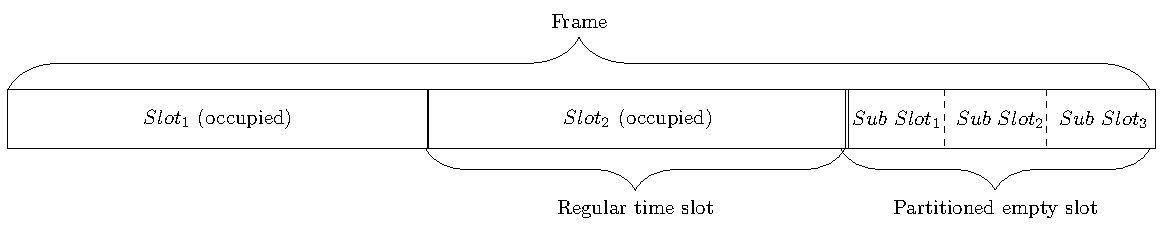
\includegraphics[width=1\textwidth]{images/subslut.pdf}
                }%
                \end{figure}
            }
        \end{frame}

        \begin{frame}[t]{Epilogue}\framesubtitle{Developed Improvements}
                    \begin{itemize}
                        \item<1-4> Frame Defragmentation
                            \begin{itemize}
                                \item<1,2> Decremental Gradual Defragmentation
                                \item<1,3> Jumping Defragmentation
                                \item<1,4> Automatic Insertion
                            \end{itemize}
                    \end{itemize}
                    \only<2>{
                    \begin{figure}
                        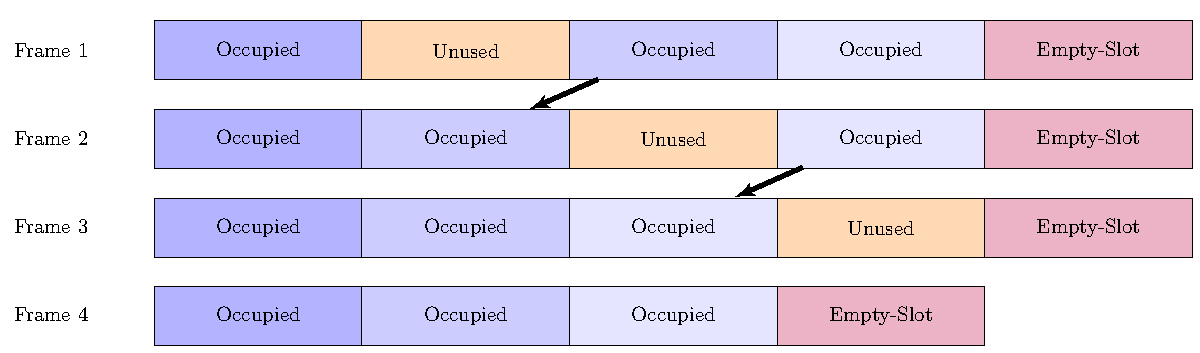
\includegraphics[width=1\textwidth]{images/dgd.pdf}
                    \end{figure}
                    }
                    \only<3>{
                    \begin{figure}
                        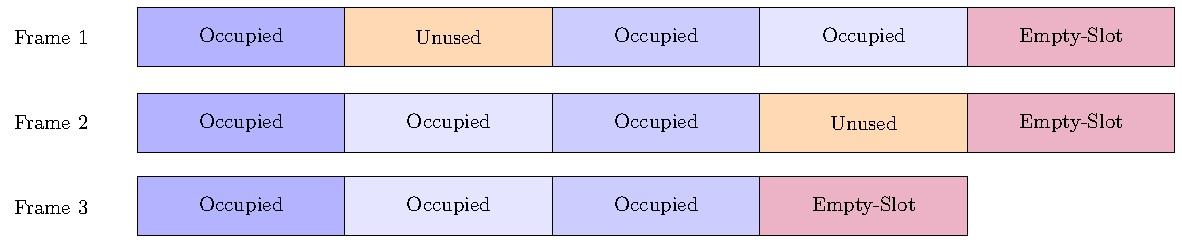
\includegraphics[width=1\textwidth]{images/jd.pdf}
                    \end{figure}
                    }
                    \only<4>{
                    \begin{figure}
                        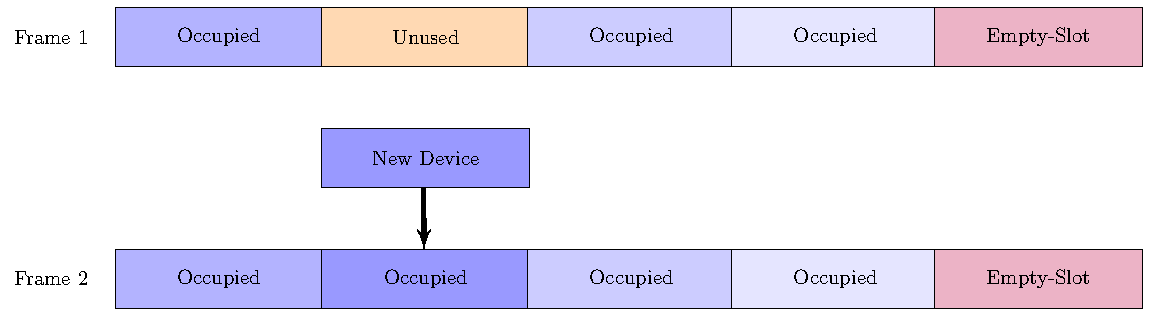
\includegraphics[width=1\textwidth]{images/aiut.pdf}
                    \end{figure}
                    }
        \end{frame}

 %       \begin{frame}[t]{Epilogue}\framesubtitle{Further Points of Interest}    
 %           \begin{itemize}
 %               \item Interrupt Library
 %               \item Operating Speed
 %                   \begin{itemize}
 %                           \item Software Improvements
 %                           \item Hardware Improvements
 %                   \end{itemize}
 %           \end{itemize}
 %       \end{frame}

    \subsection{Conclusion}
        \begin{frame}[t]{Epilogue}\framesubtitle{Conclusion}
        \begin{columns}[T]
            \begin{column}{0.48\textwidth}
                \begin{itemize}
                    \item<1-5> Development Method
                    \item<1-5> Adaptability to Reality
                        \begin{itemize}
                            \item<2-5> Uncertainty
                            \item<3-5> Physical Complications
                        \end{itemize}
                    \item<1-5> Requirements
                        \begin{itemize}
                            \item<4-5> Death Detection
                            \item<5> Echo  
                        \end{itemize}
                \end{itemize}
            \end{column}
            \begin{column}{.48\textwidth}

\begin{figure}
\centering
\resizebox{5.25cm}{!}{%
\begin{tikzpicture} [
        node distance = 1 cm,   
        vertex/.style = {circle, draw, fill=blue!10}, 
        edge/.style = {draw, -stealth, shorten >= 1pt},
        label/.style={fill=white}
    ]

    \node[draw=none](0){};
    \node[vertex, left =  3cm of 0]   (1) {$v_1$};
    \node[vertex, above=  2cm of 0]   (2) {$v_2$};
    \node[vertex, right=  3cm of 0]   (3) {$v_3$};
    \node[vertex, below=  2cm of 0]   (4) {$v_4$};
    
    \path[edge] (1) edge[bend left=15] node [label] {0.7} (2) edge[bend left=15] node [label] {0.5} (4);
    \path[edge] (1) edge[bend left=15] node [label] {0.7} (2) edge[bend left=15] node [label] {0.3} (3);
    \path[edge] (3) edge[bend left=15] node [label] {0.7} (2) edge[bend left=15] node [label] {0.3} (1);
    \path[edge] (2) edge[bend left=15] node [label] {0.7} (1) edge[bend left=15] node [label] {0.5} (4);
    \path[edge] (4) edge[bend left=15] node [label] {0.7} (1) edge[bend left=15] node [label] {0.5} (2);
    \path[edge] (2) edge[bend left=15] node [label] {0.8} (1) edge[bend left=15] node [label] {0.7} (3);
    \path[edge] (3) edge[bend left=15] node [label] {0.9} (2) edge[bend left=15] node [label] {0.1} (4);
    \path[edge] (4) edge[bend left=15] node [label] {0.4} (1) edge[bend left=15] node [label] {0.1} (3);
    
\end{tikzpicture}
}%
\end{figure}


            \end{column}
        \end{columns}
        \end{frame}

    \subsection{Future Works}
        \begin{frame}[t]{Epilogue}\framesubtitle{Strongly Connected}
            \begin{columns}[T]
                \begin{column}{0.48\textwidth}
                    \begin{itemize}
                        \item<1-4> Strongly-Connected
                        %Provides many new problems in itself, timeslot, previous work must be reconsidered etc.
                        \begin{itemize}
                            \item<2-4> Time-Slot Scheduling
                            \item<3,4> Joining the Network
                            \item<4> Network Mediating Devices
                        \end{itemize}
                        \item<1-4> Error Reconfiguration
                        \item<1-4> Beyond the Protocol
                        %Specific use case tuning, Fire Alarm, Home Automisation etc.
                    \end{itemize}
                \end{column}
            \begin{column}{.48\textwidth}
                

    \begin{figure}
    \centering
    \resizebox{0.6cm}{!}{%
        \begin{tikzpicture} [device/.style={circle, fill=blue!40, draw}]
\node[device](d1){A};
\node[device, below=of d1](d2){B};
\node[device, below=of d2](d3){C};
\node[device, below=of d3](d4){D};
\node[device, below=of d4](d5){E};

\draw (d1) -- (d2) -- (d3) -- (d4) -- (d5);
        \end{tikzpicture}
    }%
    \end{figure}
            \end{column}
        \end{columns}
        \end{frame}